%!TEX root = ../username.tex
\chapter{Results and Future Work} \label{results_future}

\section{Results} \label{results}

\subsection{The LSTM Neural Network}

% TODO discuss accuracy, use of LSTM on other music

\subsection{Markov Chains vs Random Notes}
Although the initial population's fitness is generally greater when using Markov chains create the melodies, the use of the genetic algorithm quickly negates that difference within a few generations.
There exists the possibility that the fitness of the randomly seeded population to even surpass the fitness of the Markov chain seeded population.
Since the time to generate the initial population using Markov chains is considerable, compared to using list comprehension to create random notes, the Markov chain melodies should be relegated to generating one off melodies.
% TODO insert figures showing fitness over time for random vs Markov start

\subsection{The Music and Its Uses}
See Figures ... for some samples of output from the Markov chains, and Figures ... for some samples of output from the genetic algorithm.
There are some interesting features the genetic algorithm consistently displayed: the 

\begin{figure}[h]
	\centering
	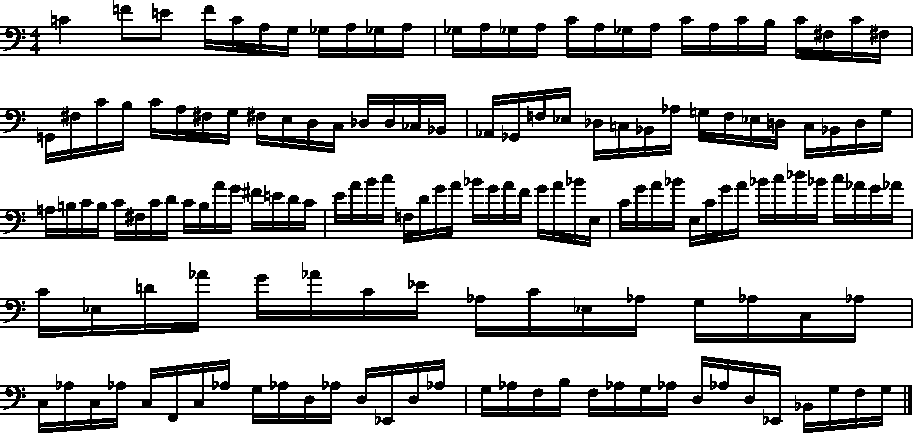
\includegraphics[width=\linewidth]{figures/markov_melody_1.pdf}
	\caption{A melody generated by Markov chains.}
	\label{fig:music:markov1}
\end{figure}

\begin{figure}[h]
	\centering
	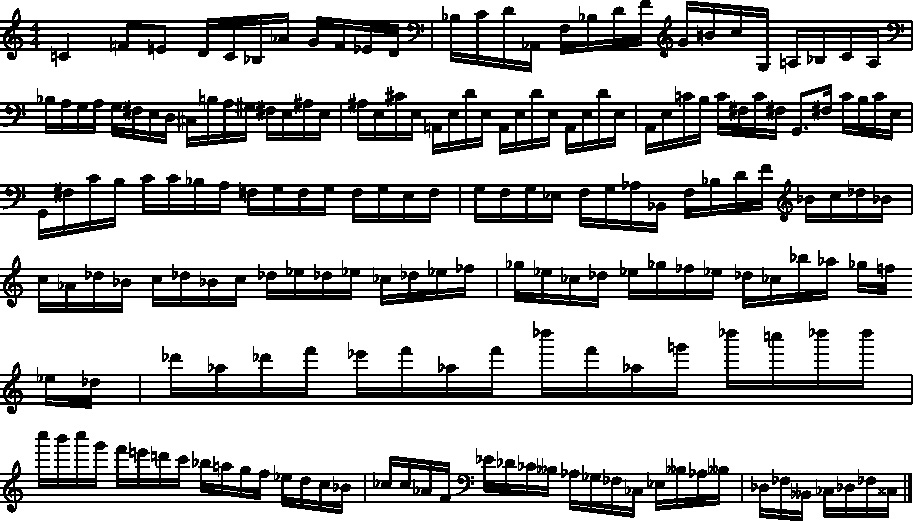
\includegraphics[width=\linewidth]{figures/markov_melody_2.pdf}
	\caption{A melody generated by Markov chains.}
	\label{fig:music:markov2}
\end{figure}

\begin{figure}[h]
	\centering
	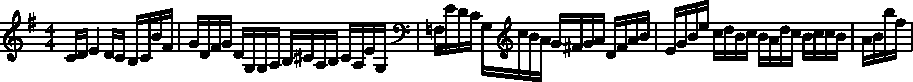
\includegraphics[width=\linewidth]{figures/genetic_melody_1.pdf}
	\caption{A melody generated with the genetic algorithm.}
	\label{fig:music:genetic}
\end{figure}

\begin{figure}[h]
	\centering
	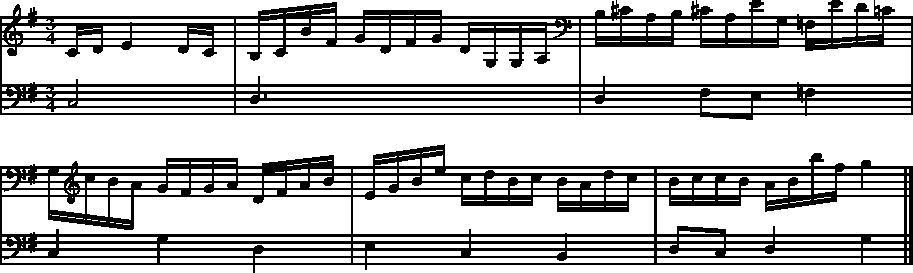
\includegraphics[width=\linewidth]{figures/genetic_melody_1_harmonized.pdf}
	\caption{The melody in Figure \ref{fig:music:genetic} with a bass line written by the author.}
	\label{fig:music:geneticHarmonized}
\end{figure}

An application of this project is to provide inspiration for the composer.
See Figure \ref{fig:music:geneticHarmonized} for an example where the author used the melody from Figure \ref{fig:music:genetic} and added a bass line.
The generated melodies could also be chained together to create longer compositions, or have their rhythms increased by some multiple.

\section{Future Work} \label{future}

The work in this paper could be expanded by writing code to generate counterpoint or harmonizations of the melodies created using the existing techniques.
Possible methods to do this might include simply using something like music21's ability to create a Roman numeral analysis of a piece to determine which chords to use.
One might also create a neural network of some variety to accept a melody and realize the bass line and other parts as desired.

There exist many machine learning algorithms that could be applied to music creation which were not explored here.
These include using convolutional neural networks, ..., and ..., to name a few.

The rhythmic generation could be enhanced to not rely so much on what pitches are played.

By expanding the project, its use could expand beyond providing musical inspiration to the composer; it could create entire works, complete with a melody, bass line, and parts in between.
